\documentclass[tikz,border=5pt]{standalone}
\usepackage[T1]{fontenc}
\usepackage{lmodern}
\usetikzlibrary{arrows.meta,positioning}
\begin{document}
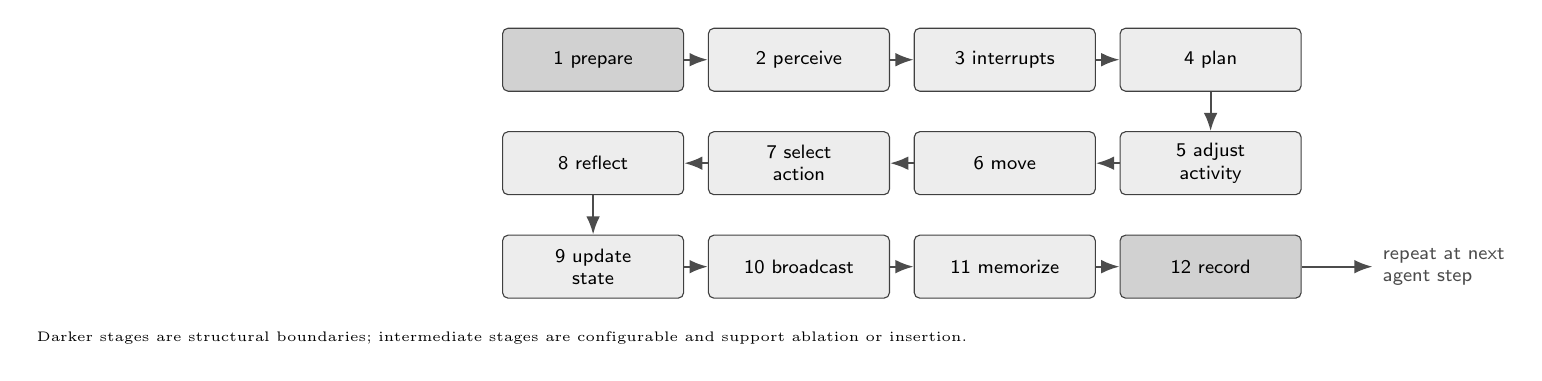
\begin{tikzpicture}[font=\sffamily\scriptsize,>=Latex,
 stage/.style={draw=black!75,rounded corners=2pt,fill=black!7,minimum width=23mm,minimum height=8mm,align=center},
 structural/.style={stage,fill=black!18}, flow/.style={->,thick,black!70}]
\node[structural] (prepare) {1 prepare};
\node[stage,right=3mm of prepare] (perceive) {2 perceive};
\node[stage,right=3mm of perceive] (interrupts) {3 interrupts};
\node[stage,right=3mm of interrupts] (plan) {4 plan};
\node[stage,below=5mm of plan] (adjust) {5 adjust\\activity};
\node[stage,left=3mm of adjust] (move) {6 move};
\node[stage,left=3mm of move] (select) {7 select\\action};
\node[stage,left=3mm of select] (reflect) {8 reflect};
\node[stage,below=5mm of reflect] (update) {9 update\\state};
\node[stage,right=3mm of update] (broadcast) {10 broadcast};
\node[stage,right=3mm of broadcast] (memorize) {11 memorize};
\node[structural,right=3mm of memorize] (record) {12 record};
\foreach \a/\b in {prepare/perceive,perceive/interrupts,interrupts/plan,plan/adjust,adjust/move,move/select,select/reflect,reflect/update,update/broadcast,broadcast/memorize,memorize/record}
  \draw[flow] (\a) -- (\b);
\draw[flow] (record.east) -- ++(9mm,0) node[right,align=left]{repeat at next\\agent step};
\node[font=\tiny,anchor=west,below=7mm of update.west] {Darker stages are structural boundaries; intermediate stages are configurable and support ablation or insertion.};
\end{tikzpicture}
\end{document}
